\section{Perturbazioni indipendenti dal tempo}
In questo capitolo si discuterà la \emph{teoria delle perturbazioni}, incominciando da quelle indipendenti dal tempo. Questo approccio allo studio di un sistema è estremamente utile in quanto consente di studiare anche sistemi non riconducibili direttamente ai problemi analiticamente più semplici da risolvere. Un classico esempio è quello dell'atomo di idrogeno: in prima istanza l'equazione di Schrödinger idrogenoide ben approssima tale sistema ma studi più approfonditi mettono in mostra la necessità di una teoria più precisa. In questo caso alcune correzioni perturbative si rivelano sufficienti a descrivere fenomeni relativistici o di carattere spin-orbita.\\

Nello studio di questi sistemi è comune suddividere l'hamiltoniano $\hat{H}$ che descrive il sistema in due termini:
\begin{itemize}
    \item $\hat{H}_0$ \emph{hamiltoniano imperturbato}, di cui è nota la soluzione del problema agli autovalori,
    \item $\hat{W}$ \emph{perturbazione}, ossia il termine che perturba il sistema.
\end{itemize}
Nel complesso l'hamiltoniano diventa:
\begin{equation}
    \hat{H}=\hat{H}_0+\hat{W}.\label{H Perturbata}
\end{equation}
SI supporrà inizialmente che $\hat{H}_0$ abbia spettro discreto.\\
Per poter utilizzare la teoria perturbata è necessario che il termine $\hat{W}$ descriva un'interazione di piccola entità rispetto all'hamiltoniano imperturbato. Per questo si definiscono tre quantità che stimano l'ordine di grandezza dei contributi energetici:
\begin{itemize}
    \item $\overline{H_0}$ che stima l'ordine di grandezza dei livelli energetici imperturbati,
    \item $\overline{\Delta H_0}$ che stima l'ordine di grandezza della separazione di due livelli imperturbati successivi,
    \item $\overline{W}$ che stima il contributo energetico dovuto alla perturbazione $\hat{W}$.
\end{itemize}
L'approccio perturbativo è adoperabile solamente se sono valide:
\begin{equation}
    \overline{H_0}\gg \overline{W}, \qquad \overline{\Delta H_0}\gg \overline{W}.
\end{equation}
Queste condizioni garantiscono che anche l'hamiltoniano perturbato abbia spettro discreto come quello imperturbato. Infatti eventuali ulteriori livelli energetici, la cui degenerazione è rimossa dalla perturbazione, per le condizioni richieste si separeranno per energie piccole rispetto a quelle del sistema imperturbato.\\

Lo stato imperturbato, come si è già detto, è di soluzione nota, fornita dall'equazione:
\begin{equation}
    \hat{H}_0\ket{n}=\ket{n}h(n),\label{schr Imperturbata}
\end{equation}
dove $\ket{n}$ è un autoket di autovalore $h(n)$. Siccome $\hat{H_0}$ è autoaggiunto e ha spettro discreto tutti i $\ket{n}$ sono ortogonali e per il principio di completezza si assume che formino una base.\\
Lo stato del sistema perturbato è determinato dalla soluzione del problema agli autovalori dell'operatore \eqref{H Perturbata}:
\begin{equation}
    \hat{H}\ket{n_p,p}=\ket{n_p,p}h(n_p,p),\label{schr Perturbata}
\end{equation}
dove $\ket{n_p,p}$ è un autoket di autovalore $h(n_p,p)$, $n_p$ rappresenta un indice che caratterizza l'autoket perturbato e $p$ indica che risolve l'equazione di Schrödinger perturbata.\\Siccome è richiesto che la perturbazione sia piccola si suppone che autoket e autovalori perturbati siano esprimibili come una serie di potenze dell'energia di perturbazione 
\begin{flalign}
    &\ket{n_p,p}=\sum_{k=0}^{\infty}\ket{n_p,k}=\ket{n_p,0}+\ket{n_p,1}+\ket{n_p,2}\dots\ ,\label{autoket perturbati}\\
    &h(n_p,p)=\sum_{k=0}^{\infty}h(n_p,k)=h(n_p,0)+h(n_p,1)+h(n_p,2)+\dots\ , \label{autovalori perturbati}
\end{flalign}
dove $\ket{n_p,k},\ h(n_p,k)$ sono di ordine $O(\overline{W}^k)$.\\

Va ora osservato che se si considera il limite fittizio\footnote{Fittizio poiché non sempre fisicamente realizzabile.} in cui la perturbazione viene eliminata dal sistema allora gli autoket perturbati \eqref{autoket perturbati} e gli autovalori perturbati \eqref{autovalori perturbati} si riducono a quelli imperturbati. Inoltre in questo caso le serie di potenze si riducono al solo termine di ordine zero:
\begin{flalign*}
    &\ket{n_p,p}=\ket{n_p,0}\longrightarrow \ket{i},\\
    &h(n_p,p)=h(n_p,0)\longrightarrow h(i) .
\end{flalign*}
Si osservi che più autoket e autovalori perturbati differenti (potendo avere identici termini di ordine $0$) possono degenerare, in assenza di perturbazione, in un unico autoket e autovalore imperturbato.
\begin{figure}[h!]
    \centering
    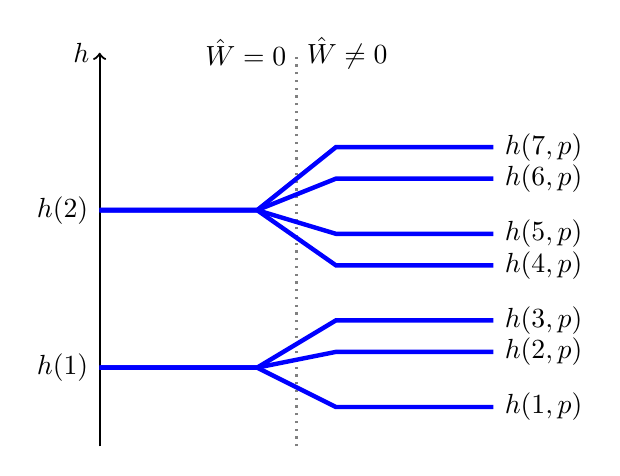
\begin{tikzpicture}
        \draw[->,thick] (0,0) -- (0,5)node[anchor=east]{$h$};
        \draw[dotted,gray,thick] (2.5,0) -- (2.5,5)node[anchor=west,black]{$\hat{W}\neq 0$}node[anchor=east,black](2.5,5){$\hat{W}= 0$};
        \draw[ultra thick, blue] (0,1)node[anchor=east,black]{$h(1)$} -- (2,1) -- (3,1.6) -- (5,1.6)node[anchor=west,black]{$h(3,p)$};
        \draw[ultra thick, blue] (0,1) -- (2,1) -- (3,1.2) -- (5,1.2)node[anchor=west,black]{$h(2,p)$};
        \draw[ultra thick, blue] (0,1) -- (2,1) -- (3,.5) -- (5,.5)node[anchor=west,black]{$h(1,p)$};
        \draw[ultra thick, blue] (0,3)node[anchor=east,black]{$h(2)$} -- (2,3) -- (3,3.8) -- (5,3.8)node[anchor=west,black]{$h(7,p)$};
        \draw[ultra thick, blue] (0,3) -- (2,3) -- (3,3.4) -- (5,3.4)node[anchor=west,black]{$h(6,p)$};
        \draw[ultra thick, blue] (0,3) -- (2,3) -- (3,2.7) -- (5,2.7)node[anchor=west,black]{$h(5,p)$};
        \draw[ultra thick, blue] (0,3) -- (2,3) -- (3,2.3) -- (5,2.3)node[anchor=west,black]{$h(4,p)$};

    \end{tikzpicture}
\end{figure}
 

\subsection{Calcolo degli stati perturbati}
Si vuole ottenere ora un metodo operativo per determinare i termini delle serie che esprimono gli autoket e gli autovalori perturbati.\\

Per procedere nell'analisi del problema perturbato è opportuno introdurre due nuovi operatori. Infatti in generale il problema impertubato può essere degenere: sia $A_i$ l'insieme degli autoket impertubati $\ket{n}$ che hanno autovalore $h(i)$.
\begin{definition}
    Si definisce autoproiettore di $h(i)$ l'operatore:
    \begin{equation}
        \hat{P}(i)=\sum_{n \in A_i}\ket{n}\bra{n}.
    \end{equation} 
\end{definition}
Questo non è altro che il proiettore ortogonale sull'autospazio di $h(i)$.
\begin{definition}
    Si definisce risolvente di $h(i)$ l'operatore:
    \begin{equation}
        \hat{D}(i)=\sum_{n\notin A_i}\frac{\ket{n}\bra{n}}{h(i)-h(n)}.
    \end{equation}
\end{definition}
Questi due operatori saranno utili nella risoluzione del problema di Schrödinger perturbato.\\
Per prima cosa è necessario dimostrare una serie di proprietà di questi due operatori.
\begin{proposition}
    Valgono le seguenti proprietà:
    \begin{flalign*}
        &\hat{H}_0\hat{P}(i)=\hat{P}(i)\hat{H}_0=h(i)\hat{P}(i),\\
        &\hat{D}(i)\hat{P}(i)=\hat{P}(i)\hat{D}(i)=0,\\
        &(h(i)\hat{I}-\hat{H}_0)\hat{D}(i)=\hat{D}(i)(h(i)\hat{I}-\hat{H}_0)=\hat{I}-\hat{P}(i).
    \end{flalign*}
\end{proposition}
\begin{proof}
    Si osservi che dalle definizioni segue:
    \begin{flalign*}
        \hat{H}_0\hat{P}(i)&=\sum_{n \in A_i}\hat{H}_0\ket{n}\bra{n}=\sum_{n \in A_i}\ket{n}h(n)\bra{n}=h(i)\sum_{n \in A_i}\ket{n}\bra{n}=h(i)\hat{P}(i).
    \end{flalign*}
    Da questa segue il resto della relazione poiché entrambi sono operatori autoaggiunti.\\

    Per dimostrare la seconda relazione è sufficiente far uso delle definizioni:
    \begin{flalign*}
        \hat{D}(i)\hat{P}(i)&=\sum_{m\notin A_i}\sum_{n \in A_i}\ket{m}\frac{\braket{m|n}}{h(i)-h(n)}\bra{n}=\sum_{m\notin A_i}\sum_{n \in A_i}\ket{m}\frac{\delta_{m,n}}{h(i)-h(n)}\bra{n}=0.
    \end{flalign*}
    Analogamente si procede per $\hat{P}(i)\hat{D}(i)$, dimostrando la seconda relazione.\\

    Per la terza relazione dalle definizioni si ha:
    \begin{flalign*}
        (h(i)\hat{I}-\hat{H}_0)\hat{D}(i)&=\sum_{n\notin A_i}(h(i)\hat{I}-\hat{H}_0)\frac{\ket{n}\bra{n}}{h(i)-h(n)}=\sum_{n\notin A_i}\ket{n}\frac{h(i)-h(n)}{h(i)-h(n)}\bra{n}\\&=\sum_{n\notin A_i}\ket{n}\bra{n}=\sum_{n}\ket{n}\bra{n}-\sum_{n\in A_i}\ket{n}\bra{n}=\hat{I}-\hat{P}(i).
    \end{flalign*}
    Da questa, usando il fatto che $\hat{H}_0$ e $\hat{D}(i)$ sono autoaggiunti, si dimostra il resto della terza relazione.
\end{proof}
Note queste proprietà si può ottenere la formula generale che consente di risolvere il problema agli autovalori perturbati. Da adesso in poi si fisserà $n_p$ e $i$ in maniera tale che $h(n_p,0)=h(i)$ e si ometteranno questi nella notazione degli operatori. Inoltre si definisce $w(n_p,p)=h(n_p,p)-h(n_p,0)=h(n_p,1)+h(n_p,2)+\dots\ $.
\begin{theorem}
    \label{thm:slz Generale Perturb Indip}
    Il problema di Schrödinger perturbato è riconducibile alla risoluzione delle seguenti equazioni operatoriali:
    \begin{flalign}
        &\hat{P}(\hat{W}+\hat{W}\sum_{n=0}^{\infty}[\hat{D}(\hat{W}-\hat{I}w)]^n\hat{D}\hat{W})\hat{P}\ket{n_p,p}=\hat{P}\ket{n_p, p}w,\\
        &\sum_{n=0}^{\infty}[\hat{D}(\hat{W}-\hat{I}w)]^n\hat{D}\hat{W})\hat{P}\ket{n_p,p}=(\hat{I}-\hat{P})\ket{n_p,p}
    \end{flalign}
\end{theorem}
Il vantaggio di queste due equazioni è quello di poter essere facilmente adoperate assieme allo sviluppo in serie degli autoket e degli autovalori.
Volendo ottenere il problema di Schrödinger approssimato al prim'ordine si inseriscono nelle relazioni del Teorema \ref{thm:slz Generale Perturb Indip} i termini perturbativi di ordine $1$ e si eliminano tutti i termini dove appaiono termini di ordine superiore:
\begin{equation}
    \boxed{\hat{P}(i)\hat{W}\hat{P}(i)\ket{n_p,0}=\ket{n_p,0}h(n_p,1)}.
\end{equation} 
Al secondo ordine invece si ottengono le due seguenti equazioni:
\begin{flalign}
    &\boxed{\hat{P}(i)(\hat{W}+\hat{W}\hat{D}(i)\hat{W})\hat{P}(i)(\ket{n_p,0}+\hat{P}(i)\ket{n_p,1})=(\ket{n_p,0}+\hat{P}(i)\ket{n_p,1})(h(n_p,1)+h(n_p,2))},\\
    &\boxed{(\hat{I}-\hat{P}(i))\ket{n_p,1}=\hat{D}(i)\hat{W}\ket{n_p,0}}.
\end{flalign}
\begin{proof}[Dimostrazione Teorema \ref{thm:slz Generale Perturb Indip}]
    Si vogliono ricavare le relazioni del Teorema \ref{thm:slz Generale Perturb Indip} dall'equazione di Schrödinger:
    \begin{flalign*}
        &[\hat{H}_0+\hat{W}]\ket{n_p,p}=\ket{n_p,p}h(n_p,p)=\ket{n_p,p}(h(i)-w(n_p,p))\\
        &\Longrightarrow [\hat{H}_0+\hat{W}-\hat{I}(h(i)-w(n_p,p)]\ket{n_p,p}=0.
    \end{flalign*}
    Utilizzando le proprietà dell'operatore $\hat{D}$ (per cui $\hat{D}(\hat{H}_0+\hat{I}h(i))=\hat{P}-\hat{I}$) e moltiplicando a sinistra l'equazione di Schrödinger per $\hat{D}$ si ha:
    \begin{equation}
       [\hat{I}-\hat{P}]\ket{n_p,p}=\hat{D}[\hat{W}-w(n_p,p)\hat{I}]\ket{n_p,p}.
    \end{equation}
    Si osservi che, scomponendo $\ket{n_p,p}$ nell'autospazio di $h(i)$ 
    \begin{equation*}
        \ket{n_p,p}=(\hat{P}+\hat{I}-\hat{P})\ket{n_p,p}
    \end{equation*}
    e inserendo questa nell'equazione precedente, si ottiene:
    \begin{equation*}
        [\hat{I}-\hat{P}]\ket{n_p,p}=\hat{D}[\hat{W}-w(n_p,p)\hat{I}](\hat{P}+\hat{I}-\hat{P})\ket{n_p,p}.
    \end{equation*}
    Questa equazione presenta due volte il termine $\hat{I}-\hat{P}$, se si sfrutta ricorsivamente questa uguaglianza si ottiene:
    \begin{equation*}
        [\hat{I}-\hat{P}]\ket{n_p,p}=\sum_{n=1}^{\infty}[\hat{D}(\hat{W}-w(n_p,p)\hat{I})]^n\hat{P}\ket{n_p,p}.
    \end{equation*}
    Ricordando la proprietà per cui $\hat{D}\hat{P}=0$ si ha l'uguaglianza: $\hat{D}(\hat{W}-w\hat{I})\hat{P}=\hat{D}\hat{W}\hat{P}$. Facendo uso di questa, nell'ultima equazione ottenuta, si ha la seconda relazione del Teorema:
    \begin{flalign*}
        [\hat{I}-\hat{P}]\ket{n_p,p}&=\sum_{n=1}^{\infty}[\hat{D}(\hat{W}-w(n_p,p)\hat{I})]^{n-1}\hat{D}\hat{W}\hat{P}\ket{n_p,p}\\
        &=\sum_{n=0}^{\infty}[\hat{D}(\hat{W}-w(n_p,p)\hat{I})]^{n}\hat{D}\hat{W}\hat{P}\ket{n_p,p}
    \end{flalign*}
    A questo punto si moltiplichi l'equazione di Schrödinger per $\hat{P}$ a sinistra, utilizzando le proprietà di questo operatore (per cui $\hat{P}(\hat{H}_0-h(i))=0$) si ottiene: 
    \begin{equation*}
        \hat{P}[\hat{W}-w(n_p,p)\hat{I}]\ket{n_p,p}=0.
    \end{equation*}
    Scomponendo $\ket{n_p,p}$ nell'autospazio di $h(i)$ questa diventa:
    \begin{equation*}
        \hat{P}[\hat{W}-w(n_p,p)\hat{I}](\hat{P}+\hat{I}-\hat{P})\ket{n_p,p}=0.
    \end{equation*}
    Si sostituisca in quest'ultima equazione il termine $[\hat{I}-\hat{P}]\ket{n_p,p}$ con la sua espressione data dalla serie precedentemente ottenuta:
    \begin{flalign*}
        [\hat{P}\hat{W}\hat{P}-w(n_p,p)\hat{P}]\ket{n_p,p}+\hat{P}[\hat{W}-w(n_p,p)\hat{I}]\sum_{n=0}^{\infty}[\hat{D}(\hat{W}-w(n_p,p)\hat{I})]^{n}\hat{D}\hat{W}\hat{P}\ket{n_p,p}=0
    \end{flalign*}
    Per concludere si osservi che per la proprietà $\hat{D}\hat{P}=0$ si ha che $\hat{D}\hat{P}\hat{W}=\hat{D}\hat{P}(\hat{W}-w\hat{I})=0$, che consente di annullare l'ultimo addendo dell'equazione sopra, così da ottenere la prima relazione:
    \begin{equation*}
        \hat{P}(\hat{W}+\hat{W}\sum_{n=0}^{\infty}[\hat{D}(\hat{W}-\hat{I}w)]^n\hat{D}\hat{W})\hat{P}\ket{n_p,p}=\hat{P}\ket{n_p, p}w.
    \end{equation*}
\end{proof}
\subsection{Sistemi perturbati non degeneri}
I risultati ottenuti dal Teorema \ref{thm:slz Generale Perturb Indip} sono di facile utilizzo nel caso in cui gli stati perturbati non degenerano, ossia quando si rimuove la perturbazione. In questo caso l'auto spazio $h(i)$ contiene un solo autoket perturbato e quindi gli operatori autoproiettore e risolvente si riducono a:
\begin{equation*}
    \hat{P}(i)=\ket{i}\bra{i},\qquad\qquad\hat{D}(i)=\sum_{n\neq i}\frac{\ket{n}\bra{n}}{h(i)-h(n)}.
\end{equation*}
I termini di ordine $0$, degli autoket e autovalori perturbati, sono autovalori e autoket imperturbati.
Prendendo $\ket{i}=\ket{n_p,0}$ ed esplicitando gli operatori nell'equazione utilizzata per calcolare le perturbazioni al prim'ordine:
\begin{flalign*}
    &\hat{P}(i)\hat{W}\hat{P}(i)\ket{n_p,0}=\ket{i}\bra{i}\hat{W}\ket{i}\bra{i}\ket{n_p,0}=\ket{n_p,0}\bra{n_p,0}\hat{W}\ket{n_p,0}=\ket{n_p,0}h(n_p,1)\\
    &\Longrightarrow \boxed{h(n_p,1)=\bra{n_p,0}\hat{W}\ket{n_p,0}}.
\end{flalign*}
Al second'ordine è più complessa la trattazione e necessita di più passaggi. Per prima cosa si consideri la prima relazione ottenuta al second'ordine e si diagonalizzi l'operatore a sinistra dell'uguale:
\begin{flalign*}
    &\hat{P}(i)(\hat{W}+\hat{W}\hat{D}(i)\hat{W})\hat{P}(i)(\ket{n_p,0}+\hat{P}(i)\ket{n_p,1})=(\ket{n_p,0}+\hat{P}(i)\ket{n_p,1})(h(n_p,1)+h(n_p,2))\\
   &=\bigg[\ket{i}\bra{i}\hat{W}(1+\sum_{n\neq i}\frac{\ket{n}\bra{n}}{h(i)-h(n)}\hat{W})\ket{i}\bra{i}\bigg](\ket{n_p,0}+\hat{P}(i)\ket{n_p,1})\\
    &=\ket{i}\bigg[\bra{i}\hat{W}\ket{i}+\sum_{n\neq i}\frac{|\braket{i|\hat{W}|n}|^2}{h(i)-h(n)}\bigg]\bra{i}(\ket{n_p,0}+\hat{P}(i)\ket{n_p,1}).
\end{flalign*}
Questa scomposizione (ricordando $\ket{i}=\ket{n_p,0}$) implica che l'autovalore:
\begin{flalign*}
    &h(n_p,1)+h(n_p,2)=\bra{i}\hat{W}\ket{i}+\sum_{n\neq i}\frac{|\braket{i|\hat{W}|n}|^2}{h(i)-h(n)}=h(n_p,1)+\sum_{n\neq i}\frac{|\braket{n_p,0|\hat{W}|n}|^2}{h(i)-h(n)}\\
    &\Longrightarrow\boxed{h(n_p,2)=\sum_{n\neq i}\frac{|\braket{n_p,0|\hat{W}|n}|^2}{h(i)-h(n)}}
\end{flalign*}
La diagonalizazione dell'operatore implica anche che $\ket{i}=\ket{n_p,0}+\hat{P}(i)\ket{n_p,1}$, come si è già detto però $\ket{i}=\ket{n_p,0}$, per cui $\hat{P}(i)\ket{n_p,1}=0$. Usando questo fatto nella seconda relazione al second'ordine si ottiene:
\begin{flalign*}
    &(\hat{I}-\hat{P}(i))\ket{n_p,1}=\hat{D}(i)\hat{W}\ket{n_p,0}=\sum_{n\neq i}\ket{n}\frac{\braket{n|\hat{W}|n_p,0}}{h(i)-h(n)}\\
    &\Rightarrow \boxed{\ket{n_p,1}=\sum_{n\neq i}\ket{n}\frac{\braket{n|\hat{W}|n_p,0}}{h(i)-h(n)}}.
\end{flalign*}
\begin{proposition}
    Il problema di Schrödinger, per perturbazioni di $\hat{H}_0$ non degenere, è approssimato al secondo ordine da:
    \begin{flalign*}
        &\ket{n_p,0}=\ket{i},\\
        &h(n_p,0)=h(i),\\
        &\ket{n_p,1}=\sum_{n\neq i}\ket{n}\frac{\braket{n|\hat{W}|n_p,0}}{h(i)-h(n)},\\
        &h(n_p,1)=\bra{n_p,0}\hat{W}\ket{n_p,0},\\
        &h(n_p,2)=\sum_{n\neq i}\frac{|\braket{n_p,0|\hat{W}|n}|^2}{h(i)-h(n)}.
    \end{flalign*}
    Dove si sono indicati $\ket{i},\ h(i)$ rispettivamente autoket e autovalore imperturbati e $\ket{n_p,k},\ h(n_p,k)$ rispettivamente autoket e autovalore perturbati di ordine $k$.
\end{proposition}
\begin{example}[Pertrubazioni di un sistema a due livelli]
    
\end{example}